% !TEX root = ../document.tex
% !TeX spellcheck = pt_BR

\section{Método de Gopalakrishnan et al.}
\label{sec:section4}
O último método implementado faz uso de uma série de resultados da álgebra linear e também da relação entre as funções de Hermite e a matriz de Fourier\footnote{matriz de Fourier é aquela que, quando multiplicada por um vetor, resulta na DFT do vetor}. Baseando-se em trabalhos anteriores \cite{Mugler02}, os autores advogam que os autovetores de uma matriz tridiagonal $T_b$ que comuta\footnote{diz-se que duas matrizes A e B comutam sse satisfizerem a condição $AB = BA$} com a matriz centralizada de Fourier equivalem às funções discretas de Hermite. Similarmente ao caso do método de Rocha et al., estas funções são utilizadas para aproximar cada batida cardíaca do registro de ECG. A figura \ref{fig:gopalak_01} mostra em linhas gerais o método proposto.

\begin{figure}[ht]
    \centering
    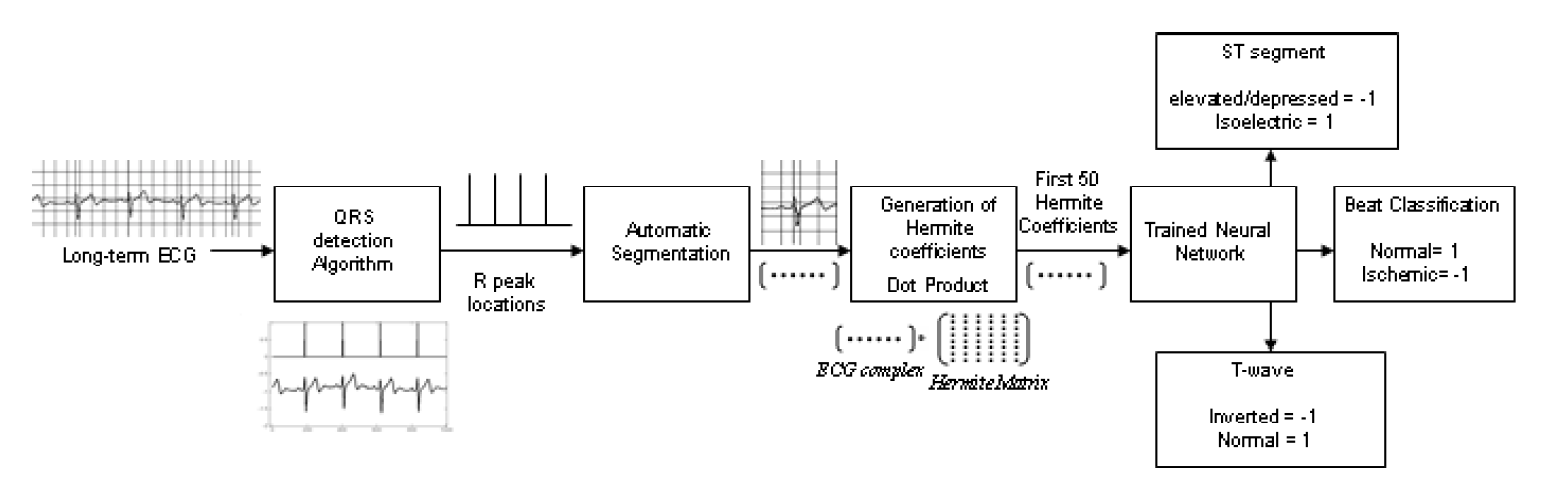
\includegraphics[width=1.0\textwidth]{figures/gopalak_01.png}
    \caption{Diagrama de blocos da estratégia utilizada no método de Gopalakrishnan et al. Extraído de \cite{Gopalak04}}
    \label{fig:gopalak_01}
\end{figure}

\subsection{Geração das funções de Hermite}
Conforme já mencionado, as funções discretas de Hermite são autovetores da matriz $T_b$. Como esta matriz é tridiagonal e simétrica, podemos descrevê-la por completo especificando sua diagonal principal e uma das diagonais secundárias. Os elementos da diagonal principal ($d^0$) e da diagonal secundária ($d^1$) são obtidos pelas expressões abaixo.
\begin{equation} \label{equ:main_diagonal}
    d^0_{i} = -2\cos(N\pi\tau)\sin(i\pi\tau)\sin((N-i-1)\pi\tau)
\end{equation}
\begin{equation} \label{equ:off_diagonal}
    d^1_{k} = \sin(k\pi\tau)\sin((N-k)\pi\tau)
\end{equation}
para $0\leq i\leq N-1$, $1\leq k\leq N-1$ e $\tau = 1/(Nb^2)$, onde $b$ é um parâmetro de dilatação e $N$ é o tamanho do sinal de entrada.

O efeito do parâmetro $b$ é um alargamento das funções de Hermite no eixo temporal, à medida que $b$ aumenta. Com um ajuste adequado, é possível aproximar de maneira fiel uma batida cardíaca sem necessitar um número elevado de funções. Mas a vantagem principal desta técnica é que existem algoritmos eficientes para o cálculo de autovetores de uma matriz tridiagonal. Além disso, os autovetores são ortogonais, o que implica que eles contêm informações independentes entre si.

As funções de Hermite de ordem $n$, em tempo contínuo, são definidas aqui como
\begin{equation} \label{equ:hermite_func2}
    \psi_n(t) = \frac{e^{-t^2/2}}{\sqrt{2^nn!\sqrt{\pi}}}H_n(t)
\end{equation}
onde $H_n(t)$ são os polinômios de Hermite, definidos pela relação de recorrência $H_0 = 1$, $H_1 = t$ e $H_k(t)=2tH_{k-1}(t)-2(k-1)H_{k-2}(t)$ para $k \geq 2$. Em tempo discreto, a função assume uma notação com a letra $u$ no lugar de $\psi$. Os autores afirmam que o índice $k=0$, do maior autovalor da matriz $T_b$, corresponde à primeira função discreta de Hermite ($u_0$), o do segundo maior autovalor, $k=1$, à segunda função ($u_1$), e assim por diante. 

Portanto, o algoritmo consiste em construir a matriz $T_b$ conforme as equações \ref{equ:main_diagonal} e \ref{equ:off_diagonal}, extrair os autovetores ($e_0, e_1 \ldots e_{N-1}$) e autovalores ($\lambda_0, \lambda_1 \ldots \lambda_{N-1}$) de $T_b$, ordenar o conjunto de autovetores em ordem decrescente de seus respectivos autovalores, e usar a lista ordenada para construção da matriz que conterá as funções de Hermite discretas. Esta matriz resultante terá a forma $H = [u_0 u_1 \cdots u_{N-1}]$, onde $u_k$ é o autovetor associado ao k-ésimo maior autovalor de $T_b$. 

\subsection{Expansão de sinais discretos}
A expansão de Hermite de um sinal discreto $x$ de tamanho $N$ é simplesmente a projeção de $x$ em cada uma das $N$ funções de Hermite que formam uma base para o espaço de $x$. Geralmente, bibliotecas de software para cálculo de autovetores já fazem a normalização destes, isto é, garantem que eles possuam norma unitária. Dessa forma, as funções obtidas no procedimento de geração visto anteriormente formam uma base ortonormal, e a expansão se resume a:
\begin{equation} \label{equ:hermite_exp2}
    x = \sum_{i=0}^{N-1} c_{i,b}\cdot u_{i,b}
\end{equation}
com coeficientes dados pelo produto interno de $x$ com as funções de Hermite:
\begin{equation} \label{equ:hermite_coeff2}
    c_{i,b} = \langle x,u_{i,b} \rangle
\end{equation}

\subsection{Preparação dos dados}
Seguindo a especificação, foi implementado o detector de complexos QRS descrito em \cite{Tompkins85}. Após obtenção dos picos de onda R, assume-se que cada batida esteja centralizada neste ponto, e que sua largura seja equivalente ao intervalo entre o seu pico e o da batida seguinte (também chamado intervalo R-R). Para cada batida, os primeiros 50 coeficientes de Hermite são obtidos através da equação (\ref{equ:hermite_coeff2}). São estes coeficientes que compõem a entrada da rede neural que classificará a batida.

Os autores explicam, baseando-se em trabalhos passados e também pela observação do Erro RMS Percentual, que o uso dos primeiros 50 coeficientes, bem como de um parâmetro de dilatação $b=1$, garantem uma aproximação muito boa. Na implementação, contudo, verificou-se que o valor 1,5 para o parâmetro $b$ gera resultados melhores, e foi portanto utilizado. Mas  manteve-se o número de coeficientes de Hermite ($m=50$).

\subsection{Código MATLAB}
No trecho de código abaixo, pode-se notar uma maior simplicidade em relação aos demais métodos. Não há qualquer tratamento de anomalias ou de PVCs. Até mesmo as rotinas de filtragem e remoção da linha de base tiveram que ser implementadas à parte, porquanto não foram mencionadas pelos autores. Utilizou-se um filtro passa-banda de Butterworth de 4\textordfeminine{} ordem com frequências de corte 0,5Hz e 40Hz. Após a filtragem, estima-se o nível de base como a média dos mínimos do sinal, e subtrai-se este valor do próprio sinal.

\lstinputlisting[
    label=lst:gopalak,
    caption={Trecho extraído do arquivo gopalak.m}
]{listings/gopalak.m}
